%%%% CAPÍTULO 3 - ESPECIFICAÇÃO DO SISTEMA
%%
%% Conteúdo extraído VERBATIM de TCC_PARKON_V3.pdf (páginas 12 a 19).
%% Fragmento LaTeX: incluído via \include em tese.tex (sem preâmbulo).
%% Codificação UTF-8.
%%
%% Observações de migração:
%% - Não há citações bibliográficas ([n]) no corpo deste capítulo.
%% - Não há citações diretas com mais de três linhas (nenhum bloco \quoting é necessário).
%% - Não há pseudocódigo/algoritmos neste capítulo (nenhum ambiente \algorithm é necessário).
%% - Referência cruzada "Figura 1" convertida para \autoref{fig:caso-uso-usuario}.
%% - Figuras (Figura 1, 2 e 3): inseridos AMBIENTES PLACEHOLDER com \label para que
%%   os \autoref resolvam; as imagens reais serão extraídas/inseridas na tarefa 5.1.
%% - Tabelas (Tabela 1 a 8): criadas com \label (tab:); estrutura/refino na tarefa 5.2.
%% - Acrônimos: "API" provavelmente já introduzido no Capítulo 2 (seção 2.3 - Tecnologias
%%   Necessárias). Aqui em RNF07 usa-se \acrshortpl{api} (ocorrência subsequente, plural).
%%   A reconciliação de primeiro uso entre capítulos é feita na tarefa 10.1.
%% - Os códigos de requisito "RF01..RF06" e "RNF01..RNF07" são mantidos como
%%   identificadores literais para preservar o conteúdo VERBATIM (Req. 1.1). Os acrônimos
%%   rf/rnf estão definidos em acronimos.tex; sua inclusão na "Lista de Abreviaturas e
%%   Siglas" será tratada nas tarefas 8.1/10.1 (evitar \acrfull aqui alteraria o texto
%%   visível dos códigos).

\chapter{Especificação do Sistema}
\label{cap:proposta}

Considerando que o Parkon é uma plataforma voltada para facilitar a reserva de vagas de estacionamento, sua utilização deve ser intuitiva e acessível para diferentes perfis de usuários. Os requisitos funcionais e não funcionais são fundamentais no desenvolvimento do sistema, pois definem o escopo e a qualidade do produto. Os requisitos funcionais estabelecem as principais funcionalidades que a plataforma deve oferecer, enquanto os requisitos não funcionais determinam critérios de desempenho, segurança e usabilidade. A definição clara desses requisitos é essencial para garantir o sucesso do projeto e a satisfação dos usuários.


\section{Escopo de Utilização}
\label{sec:escopo}

O Parkon foi desenvolvido para facilitar a reserva de vagas de estacionamento em ambientes urbanos. O sistema pode ser utilizado em diferentes cenários, como estacionamentos comerciais, residenciais, públicos ou privados. Os usuários do sistema são divididos em dois perfis: motoristas, que buscam e reservam vagas por meio do aplicativo mobile, e gestores de estacionamento, que cadastram e gerenciam suas vagas e reservas por meio do portal web administrativo.


\section{Análise de Requisitos}
\label{sec:analise-requisitos}

\begin{table}[H]
\begin{center}
\caption{Requisitos Funcionais do Usuário}
\label{tab:requisitos-funcionais}
\begin{tabular}{|c|p{11cm}|}
\hline
\textbf{RF01} & Cadastro de Usuário: Permitir que novos usuários se cadastrem na plataforma, informando dados pessoais e de contato \\
\hline
\textbf{RF02} & Login e Autenticação: Permitir que usuários façam login de forma segura. \\
\hline
\textbf{RF03} & Localização de Vagas: Exibir em tempo real as vagas de estacionamento disponíveis próximas ao usuário, utilizando geolocalização. \\
\hline
\textbf{RF04} & Reserva de Vaga: Permitir que o usuário selecione e reserve uma vaga antecipadamente. \\
\hline
\textbf{RF05} & Avaliação de Vaga/Serviço: Permitir que o usuário avalie a vaga e o serviço após a utilização. \\
\hline
\textbf{RF06} & Geração de Rotas: Fornecer ao usuário a rota até o estacionamento selecionado. \\
\hline
\textbf{RF07} & Responder Comentários: Permitir que o usuário responda a comentários realizados em estacionamentos. \\
\hline
\end{tabular}
\end{center}
\end{table}

\begin{table}[H]
\begin{center}
\caption{Requisitos Funcionais do Administrador do Estacionamento}
\label{tab:requisitos-funcionais-admin}
\begin{tabular}{|c|p{11cm}|}
\hline
\textbf{RF08} & Cadastro do Administrador: Permitir que gestores de estacionamento se cadastrem na plataforma web. \\
\hline
\textbf{RF09} & Login do Administrador: Permitir que o administrador faça login de forma segura no portal web. \\
\hline
\textbf{RF10} & Cadastrar/Editar Empresa: Permitir que o administrador cadastre e edite os dados da empresa responsável pelo estacionamento. \\
\hline
\textbf{RF11} & Cadastrar Estacionamento: Permitir que o administrador cadastre um ou mais estacionamentos vinculados à empresa. \\
\hline
\textbf{RF12} & Configurar Estacionamento: Permitir que o administrador configure informações do estacionamento, como quantidade de vagas, horários de funcionamento e preços. \\
\hline
\textbf{RF13} & Adicionar Colaboradores: Permitir que o administrador adicione outros colaboradores para auxiliar na gestão do estacionamento. \\
\hline
\textbf{RF14} & Visualizar Reservas: Permitir que o administrador visualize as reservas realizadas pelos usuários em seus estacionamentos. \\
\hline
\textbf{RF15} & Confirmar ou Cancelar Reservas: Permitir que o administrador confirme ou cancele reservas de vagas em seus estacionamentos. \\
\hline
\textbf{RF16} & Gerenciar Informações do Estacionamento: Permitir que o administrador atualize informações gerais do estacionamento, como endereço, fotos e descrição. \\
\hline
\end{tabular}
\end{center}
\end{table}

\begin{table}[H]
\begin{center}
\caption{Requisitos Não-Funcionais}
\label{tab:requisitos-nao-funcionais}
\begin{tabular}{|c|p{11cm}|}
\hline
\textbf{RNF01} & Usabilidade: A interface do aplicativo deve ser intuitiva e acessível para usuários de diferentes perfis. \\
\hline
\textbf{RNF02} & Segurança: Os dados dos usuários e transações financeiras devem ser protegidos por mecanismos de autenticação e criptografia. \\
\hline
\textbf{RNF03} & Disponibilidade: O sistema deve estar disponível para acesso 24 horas por dia, 7 dias por semana. \\
\hline
\textbf{RNF04} & Desempenho: As informações sobre vagas disponíveis devem ser atualizadas em tempo real, com tempo de resposta inferior a 2 segundos. \\
\hline
\textbf{RNF05} & Compatibilidade: O aplicativo deve ser compatível com os principais sistemas operacionais móveis (Android e iOS). \\
\hline
\textbf{RNF06} & Escalabilidade: O sistema deve suportar o aumento do número de usuários e estacionamentos cadastrados sem perda de desempenho. \\
\hline
\textbf{RNF07} & Interoperabilidade: O sistema deve permitir integração com \acrshortpl{api} de terceiros, como sistemas de pagamento e mapas. \\
\hline
\end{tabular}
\end{center}
\end{table}


\section{Caso de Uso}
\label{sec:caso-de-uso}

\subsection{Diagramas de Casos de Uso}
\label{sec:diagramas-casos-uso}

Nesta seção, detalhamos os principais eventos que podem ocorrer dentro da plataforma Parkon, considerando os dois atores principais: o usuário motorista, que utiliza o aplicativo mobile para buscar e reservar vagas, e o administrador do estacionamento, que gerencia suas vagas e reservas por meio do portal web administrativo.

Para cada ação realizada pelo usuário, um conjunto de processos é desencadeado, afetando tanto o motorista que faz a reserva quanto o estacionamento que oferece a vaga. O diagrama da \autoref{fig:caso-uso-usuario} representa os casos de uso do usuário do sistema, enquanto o diagrama da \autoref{fig:caso-uso-administrador} apresenta os casos de uso do administrador do estacionamento.

\begin{figure}[H]
   \centering
   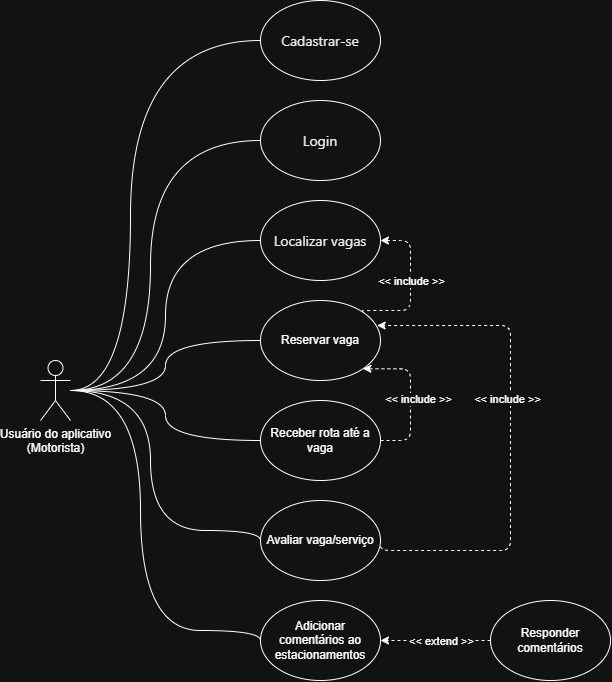
\includegraphics[width=0.6\linewidth]{capitulos/figuras/caso-uso-usuario.png}
   \caption{Diagrama de Caso de Uso do Usuário.}
   \label{fig:caso-uso-usuario}
\end{figure}

\begin{figure}[H]
   \centering
   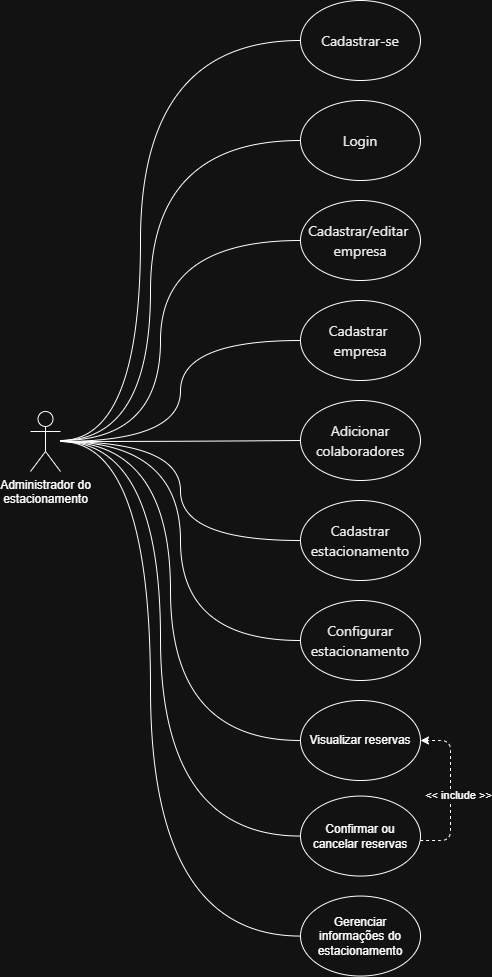
\includegraphics[width=0.6\linewidth]{capitulos/figuras/caso-uso-administrador.png}
   \caption{Diagrama de Caso de Uso do Administrador do Estacionamento.}
   \label{fig:caso-uso-administrador}
\end{figure}


\subsection{Descrição de Casos de Uso}
\label{sec:descricao-casos-uso}

A seguir, descrevemos os principais casos de uso da plataforma Parkon, organizados por ator: o usuário motorista, que utiliza o aplicativo mobile, e o administrador do estacionamento, que gerencia suas operações por meio do portal web.

\subsubsection{Casos de Uso do Usuário (Motorista)}
\label{sec:casos-uso-usuario}

Os casos de uso a seguir descrevem as principais interações do motorista com o aplicativo mobile.

\begin{table}[H]
\begin{center}
\caption{Caso de uso cadastrar-se (Motorista)}
\label{tab:caso-uso-cadastrar}
\begin{tabular}{|p{4cm}|p{9cm}|}
\hline
\textbf{Nome} & Cadastrar-se \\
\hline
\textbf{Objetivos} & Realizar cadastro de usuário na plataforma \\
\hline
\textbf{Atores} & Usuário motorista \\
\hline
\textbf{Pré-Condições} & Não existir cadastro anterior para o mesmo e-mail. \\
\hline
\textbf{Evento Chave (Trigger)} & Abertura do aplicativo pela primeira vez. \\
\hline
\textbf{Fluxo Principal} & 1. Usuário abre o aplicativo. 2. Usuário preenche formulário de cadastro. 3. Usuário clica no botão de cadastrar 4. Usuário é redirecionado para tela de Diálogos. \\
\hline
\textbf{Fluxo Alternativo} & 1. Usuário já está cadastrado. 2. Mensagem para cadastrar com outro e-mail é exibida. \\
\hline
\textbf{Pós-Condições} & Usuário cadastrado no sistema. \\
\hline
\textbf{Regras de Negócios} & Só pode existir um cadastro por e-mail. \\
\hline
\end{tabular}
\end{center}
\end{table}

\begin{table}[H]
\begin{center}
\caption{Caso de uso Login (Motorista)}
\label{tab:caso-uso-login}
\begin{tabular}{|p{4cm}|p{9cm}|}
\hline
\textbf{Nome} & Login \\
\hline
\textbf{Objetivos} & Realizar login na plataforma \\
\hline
\textbf{Atores} & Usuário motorista \\
\hline
\textbf{Pré-Condições} & Ter realizado cadastrado na plataforma anteriormente. \\
\hline
\textbf{Evento Chave (Trigger)} & \\
\hline
\textbf{Fluxo Principal} & 1. Usuário abre o aplicativo. 2. Usuário preenche informações de login. 3. Usuário é redirecionado para tela inícial \\
\hline
\textbf{Fluxo Alternativo} & 1. Usuário não cadastrado. 2. Mensagem para cadastrar é exibida. \\
\hline
\textbf{Pós-Condições} & Usuário autenticado no sistema. \\
\hline
\textbf{Regras de Negócios} & \\
\hline
\end{tabular}
\end{center}
\end{table}

\begin{table}[H]
\begin{center}
\caption{Caso de uso localizar vaga}
\label{tab:caso-uso-localizar-vaga}
\begin{tabular}{|p{4cm}|p{9cm}|}
\hline
\textbf{Nome} & Localizar Vaga \\
\hline
\textbf{Objetivos} & Encontrar estacionamentos na região informada \\
\hline
\textbf{Atores} & Usuário motorista \\
\hline
\textbf{Pré-Condições} & Ter realizado login na plataforma anteriormente. \\
\hline
\textbf{Evento Chave (Trigger)} & Pesquisa do endereço destino \\
\hline
\textbf{Fluxo Principal} & 1. Usuário informa endereço. 2. Usuário recebe lista de estacionamentos. \\
\hline
\textbf{Fluxo Alternativo} & 1. Endereço não encontrado. 2. Mensagem para informar que está incorreto é exibida. \\
\hline
\textbf{Pós-Condições} & \\
\hline
\textbf{Regras de Negócios} & \\
\hline
\end{tabular}
\end{center}
\end{table}

\begin{table}[H]
\begin{center}
\caption{Caso de uso reservar vaga}
\label{tab:caso-uso-reservar-vaga}
\begin{tabular}{|p{4cm}|p{9cm}|}
\hline
\textbf{Nome} & Reservar Vaga \\
\hline
\textbf{Objetivos} & Realizar a reserva de uma vaga no estacionamento selecionado \\
\hline
\textbf{Atores} & Usuário motorista \\
\hline
\textbf{Pré-Condições} & Ter localizado um estacionamento com vagas disponíveis. \\
\hline
\textbf{Evento Chave (Trigger)} & Seleção do estacionamento desejado \\
\hline
\textbf{Fluxo Principal} & 1. Usuário seleciona o estacionamento. 2. Usuário solicita a reserva da vaga. 3. Sistema registra a reserva com status pendente. 4. Administrador do estacionamento confirma a reserva. 5. Usuário é notificado da confirmação. \\
\hline
\textbf{Fluxo Alternativo} & 1. Administrador cancela a reserva. 2. Usuário é notificado do cancelamento. \\
\hline
\textbf{Pós-Condições} & Vaga reservada após aprovação do administrador. \\
\hline
\textbf{Regras de Negócios} & A vaga só é disponibilizada ao usuário após revisão e confirmação do administrador do estacionamento. \\
\hline
\end{tabular}
\end{center}
\end{table}

\begin{table}[H]
\begin{center}
\caption{Caso de uso receber rota até a vaga}
\label{tab:caso-uso-receber-rota}
\begin{tabular}{|p{4cm}|p{9cm}|}
\hline
\textbf{Nome} & Receber rota até a vaga \\
\hline
\textbf{Objetivos} & Obter a rota até o estacionamento encontrado \\
\hline
\textbf{Atores} & Usuário motorista \\
\hline
\textbf{Pré-Condições} & Ter encontrado um estacionamento na busca \\
\hline
\textbf{Evento Chave (Trigger)} & \\
\hline
\textbf{Fluxo Principal} & 1. Usuário encontra estacionamento 2. Sistema abre o google maps no dispositivo do cliente com a rota definida. \\
\hline
\textbf{Fluxo Alternativo} & \\
\hline
\textbf{Pós-Condições} & Usuário com rota definida no google maps \\
\hline
\textbf{Regras de Negócios} & \\
\hline
\end{tabular}
\end{center}
\end{table}

\begin{table}[H]
\begin{center}
\caption{Caso de uso avaliar vaga/serviço}
\label{tab:caso-uso-avaliar}
\begin{tabular}{|p{4cm}|p{9cm}|}
\hline
\textbf{Nome} & Avaliar vaga/serviço \\
\hline
\textbf{Objetivos} & Usuário avaliar a vaga \\
\hline
\textbf{Atores} & Usuário motorista \\
\hline
\textbf{Pré-Condições} & Ter realizado viagem até a vaga \\
\hline
\textbf{Evento Chave (Trigger)} & \\
\hline
\textbf{Fluxo Principal} & 1. Usuário finaliza rota. 2. Usuário realiza avaliação da vaga. \\
\hline
\textbf{Fluxo Alternativo} & \\
\hline
\textbf{Pós-Condições} & Nota do estacionamento é recalculada \\
\hline
\textbf{Regras de Negócios} & \\
\hline
\end{tabular}
\end{center}
\end{table}

\begin{table}[H]
\begin{center}
\caption{Caso de uso adicionar comentários ao estacionamento}
\label{tab:caso-uso-comentarios}
\begin{tabular}{|p{4cm}|p{9cm}|}
\hline
\textbf{Nome} & Adicionar comentários ao estacionamento \\
\hline
\textbf{Objetivos} & Usuário adiciona comentários sobre o estacionamento \\
\hline
\textbf{Atores} & Usuário motorista \\
\hline
\textbf{Pré-Condições} & Estar logado na plataforma \\
\hline
\textbf{Evento Chave (Trigger)} & \\
\hline
\textbf{Fluxo Principal} & 1. Usuário envia comentário do estacionamento. \\
\hline
\textbf{Fluxo Alternativo} & \\
\hline
\textbf{Pós-Condições} & Lista de comentários é atualizada \\
\hline
\textbf{Regras de Negócios} & \\
\hline
\end{tabular}
\end{center}
\end{table}

\begin{table}[H]
\begin{center}
\caption{Caso de uso responder comentários}
\label{tab:caso-uso-responder-comentarios}
\begin{tabular}{|p{4cm}|p{9cm}|}
\hline
\textbf{Nome} & Responder comentários \\
\hline
\textbf{Objetivos} & Permitir que o usuário responda a comentários em estacionamentos \\
\hline
\textbf{Atores} & Usuário motorista \\
\hline
\textbf{Pré-Condições} & Estar logado na plataforma e existir comentários no estacionamento \\
\hline
\textbf{Evento Chave (Trigger)} & Usuário acessa a seção de comentários de um estacionamento \\
\hline
\textbf{Fluxo Principal} & 1. Usuário acessa os comentários do estacionamento. 2. Usuário seleciona um comentário existente. 3. Usuário redige e envia a resposta. \\
\hline
\textbf{Fluxo Alternativo} & \\
\hline
\textbf{Pós-Condições} & Resposta é exibida vinculada ao comentário original \\
\hline
\textbf{Regras de Negócios} & \\
\hline
\end{tabular}
\end{center}
\end{table}

\subsubsection{Casos de Uso do Administrador do Estacionamento}
\label{sec:casos-uso-administrador}

Os casos de uso a seguir descrevem as principais interações do administrador com o portal web administrativo.

\begin{table}[H]
\begin{center}
\caption{Caso de uso cadastrar-se (Administrador)}
\label{tab:caso-uso-cadastrar-admin}
\begin{tabular}{|p{4cm}|p{9cm}|}
\hline
\textbf{Nome} & Cadastrar-se \\
\hline
\textbf{Objetivos} & Realizar cadastro do administrador na plataforma web \\
\hline
\textbf{Atores} & Administrador do estacionamento \\
\hline
\textbf{Pré-Condições} & Não existir cadastro anterior para o mesmo e-mail. \\
\hline
\textbf{Evento Chave (Trigger)} & Acesso ao portal web pela primeira vez \\
\hline
\textbf{Fluxo Principal} & 1. Administrador acessa o portal web. 2. Administrador preenche formulário de cadastro. 3. Administrador confirma o e-mail. 4. Administrador é redirecionado para o painel principal. \\
\hline
\textbf{Fluxo Alternativo} & 1. E-mail já cadastrado. 2. Mensagem informando cadastro existente é exibida. \\
\hline
\textbf{Pós-Condições} & Administrador cadastrado no sistema. \\
\hline
\textbf{Regras de Negócios} & Só pode existir um cadastro por e-mail e por CPF. \\
\hline
\end{tabular}
\end{center}
\end{table}

\begin{table}[H]
\begin{center}
\caption{Caso de uso Login (Administrador)}
\label{tab:caso-uso-login-admin}
\begin{tabular}{|p{4cm}|p{9cm}|}
\hline
\textbf{Nome} & Login \\
\hline
\textbf{Objetivos} & Realizar login no portal web administrativo \\
\hline
\textbf{Atores} & Administrador do estacionamento \\
\hline
\textbf{Pré-Condições} & Ter realizado cadastro na plataforma anteriormente. \\
\hline
\textbf{Evento Chave (Trigger)} & \\
\hline
\textbf{Fluxo Principal} & 1. Administrador acessa o portal web. 2. Administrador preenche informações de login. 3. Administrador é redirecionado para o painel principal. \\
\hline
\textbf{Fluxo Alternativo} & 1. Administrador não cadastrado. 2. Mensagem para cadastrar é exibida. \\
\hline
\textbf{Pós-Condições} & Administrador autenticado no sistema. \\
\hline
\textbf{Regras de Negócios} & \\
\hline
\end{tabular}
\end{center}
\end{table}

\begin{table}[H]
\begin{center}
\caption{Caso de uso cadastrar/editar empresa}
\label{tab:caso-uso-cadastrar-empresa}
\begin{tabular}{|p{4cm}|p{9cm}|}
\hline
\textbf{Nome} & Cadastrar/Editar Empresa \\
\hline
\textbf{Objetivos} & Cadastrar ou editar os dados da empresa responsável pelo estacionamento \\
\hline
\textbf{Atores} & Administrador do estacionamento \\
\hline
\textbf{Pré-Condições} & Estar autenticado no portal web. \\
\hline
\textbf{Evento Chave (Trigger)} & Acesso à seção de empresa no painel \\
\hline
\textbf{Fluxo Principal} & 1. Administrador acessa a seção de empresa. 2. Administrador preenche ou edita os dados (razão social, CNPJ, endereço). 3. Sistema valida e salva as informações. \\
\hline
\textbf{Fluxo Alternativo} & 1. Dados inválidos. 2. Mensagem de erro é exibida solicitando correção. \\
\hline
\textbf{Pós-Condições} & Empresa cadastrada ou atualizada no sistema. \\
\hline
\textbf{Regras de Negócios} & CNPJ deve ser válido e único na plataforma. \\
\hline
\end{tabular}
\end{center}
\end{table}

\begin{table}[H]
\begin{center}
\caption{Caso de uso cadastrar estacionamento}
\label{tab:caso-uso-cadastrar-estacionamento}
\begin{tabular}{|p{4cm}|p{9cm}|}
\hline
\textbf{Nome} & Cadastrar Estacionamento \\
\hline
\textbf{Objetivos} & Cadastrar um novo estacionamento vinculado à empresa \\
\hline
\textbf{Atores} & Administrador do estacionamento \\
\hline
\textbf{Pré-Condições} & Estar autenticado e possuir empresa cadastrada. \\
\hline
\textbf{Evento Chave (Trigger)} & Acesso à seção de estacionamentos no painel \\
\hline
\textbf{Fluxo Principal} & 1. Administrador acessa a seção de estacionamentos. 2. Administrador preenche dados do estacionamento (nome, endereço, capacidade). 3. Sistema valida e cadastra o estacionamento. \\
\hline
\textbf{Fluxo Alternativo} & 1. Endereço já cadastrado por outra empresa. 2. Mensagem informando conflito é exibida. \\
\hline
\textbf{Pós-Condições} & Estacionamento cadastrado e visível para os usuários do aplicativo. \\
\hline
\textbf{Regras de Negócios} & Um estacionamento deve estar vinculado a uma empresa. \\
\hline
\end{tabular}
\end{center}
\end{table}

\begin{table}[H]
\begin{center}
\caption{Caso de uso configurar estacionamento}
\label{tab:caso-uso-configurar-estacionamento}
\begin{tabular}{|p{4cm}|p{9cm}|}
\hline
\textbf{Nome} & Configurar Estacionamento \\
\hline
\textbf{Objetivos} & Definir configurações operacionais do estacionamento \\
\hline
\textbf{Atores} & Administrador do estacionamento \\
\hline
\textbf{Pré-Condições} & Estar autenticado e possuir estacionamento cadastrado. \\
\hline
\textbf{Evento Chave (Trigger)} & Acesso às configurações do estacionamento \\
\hline
\textbf{Fluxo Principal} & 1. Administrador acessa as configurações do estacionamento. 2. Administrador define quantidade de vagas, horários de funcionamento e preços. 3. Sistema salva as configurações. \\
\hline
\textbf{Fluxo Alternativo} & \\
\hline
\textbf{Pós-Condições} & Configurações aplicadas e refletidas no aplicativo mobile. \\
\hline
\textbf{Regras de Negócios} & Quantidade de vagas deve ser maior que zero. \\
\hline
\end{tabular}
\end{center}
\end{table}

\begin{table}[H]
\begin{center}
\caption{Caso de uso adicionar colaboradores}
\label{tab:caso-uso-adicionar-colaboradores}
\begin{tabular}{|p{4cm}|p{9cm}|}
\hline
\textbf{Nome} & Adicionar Colaboradores \\
\hline
\textbf{Objetivos} & Adicionar outros usuários como colaboradores na gestão do estacionamento \\
\hline
\textbf{Atores} & Administrador do estacionamento \\
\hline
\textbf{Pré-Condições} & Estar autenticado e possuir estacionamento cadastrado. \\
\hline
\textbf{Evento Chave (Trigger)} & Acesso à seção de colaboradores \\
\hline
\textbf{Fluxo Principal} & 1. Administrador acessa a seção de colaboradores. 2. Administrador informa o e-mail do colaborador. 3. Sistema envia convite ao colaborador. \\
\hline
\textbf{Fluxo Alternativo} & 1. E-mail não encontrado. 2. Convite é enviado para cadastro na plataforma. \\
\hline
\textbf{Pós-Condições} & Colaborador vinculado ao estacionamento com permissões de gestão. \\
\hline
\textbf{Regras de Negócios} & \\
\hline
\end{tabular}
\end{center}
\end{table}

\begin{table}[H]
\begin{center}
\caption{Caso de uso visualizar reservas}
\label{tab:caso-uso-visualizar-reservas}
\begin{tabular}{|p{4cm}|p{9cm}|}
\hline
\textbf{Nome} & Visualizar Reservas \\
\hline
\textbf{Objetivos} & Visualizar as reservas realizadas pelos usuários \\
\hline
\textbf{Atores} & Administrador do estacionamento \\
\hline
\textbf{Pré-Condições} & Estar autenticado e possuir estacionamento cadastrado. \\
\hline
\textbf{Evento Chave (Trigger)} & Acesso à seção de reservas no painel \\
\hline
\textbf{Fluxo Principal} & 1. Administrador acessa a seção de reservas. 2. Sistema exibe lista de reservas ativas e históricas. \\
\hline
\textbf{Fluxo Alternativo} & 1. Nenhuma reserva encontrada. 2. Mensagem informativa é exibida. \\
\hline
\textbf{Pós-Condições} & \\
\hline
\textbf{Regras de Negócios} & \\
\hline
\end{tabular}
\end{center}
\end{table}

\begin{table}[H]
\begin{center}
\caption{Caso de uso confirmar ou cancelar reservas}
\label{tab:caso-uso-confirmar-cancelar-reservas}
\begin{tabular}{|p{4cm}|p{9cm}|}
\hline
\textbf{Nome} & Confirmar ou Cancelar Reservas \\
\hline
\textbf{Objetivos} & Gerenciar o status das reservas recebidas \\
\hline
\textbf{Atores} & Administrador do estacionamento \\
\hline
\textbf{Pré-Condições} & Existir reserva pendente no estacionamento. \\
\hline
\textbf{Evento Chave (Trigger)} & Nova reserva recebida \\
\hline
\textbf{Fluxo Principal} & 1. Administrador visualiza reserva pendente. 2. Administrador confirma ou cancela a reserva. 3. Sistema notifica o usuário sobre o status. \\
\hline
\textbf{Fluxo Alternativo} & \\
\hline
\textbf{Pós-Condições} & Reserva atualizada e usuário notificado. \\
\hline
\textbf{Regras de Negócios} & Reservas canceladas devem liberar a vaga imediatamente. \\
\hline
\end{tabular}
\end{center}
\end{table}

\begin{table}[H]
\begin{center}
\caption{Caso de uso gerenciar informações do estacionamento}
\label{tab:caso-uso-gerenciar-info}
\begin{tabular}{|p{4cm}|p{9cm}|}
\hline
\textbf{Nome} & Gerenciar Informações do Estacionamento \\
\hline
\textbf{Objetivos} & Atualizar informações gerais do estacionamento \\
\hline
\textbf{Atores} & Administrador do estacionamento \\
\hline
\textbf{Pré-Condições} & Estar autenticado e possuir estacionamento cadastrado. \\
\hline
\textbf{Evento Chave (Trigger)} & Necessidade de atualizar dados do estacionamento \\
\hline
\textbf{Fluxo Principal} & 1. Administrador acessa as informações do estacionamento. 2. Administrador edita dados como endereço, fotos, descrição e contato. 3. Sistema valida e salva as alterações. \\
\hline
\textbf{Fluxo Alternativo} & 1. Dados inválidos. 2. Mensagem de erro é exibida. \\
\hline
\textbf{Pós-Condições} & Informações atualizadas e refletidas no aplicativo mobile. \\
\hline
\textbf{Regras de Negócios} & \\
\hline
\end{tabular}
\end{center}
\end{table}


\section{Modelagem do Sistema}
\label{sec:modelagem-sistema}

\begin{figure}[H]
   \centering
   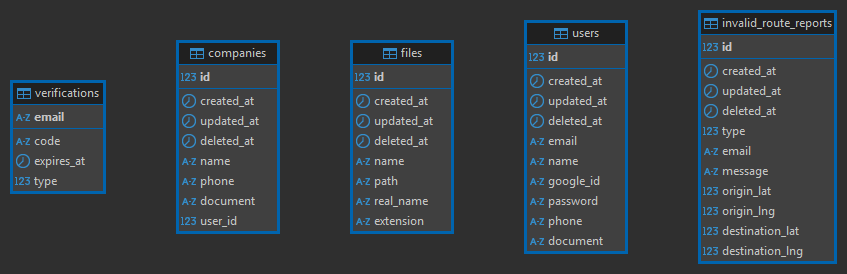
\includegraphics[width=0.95\linewidth]{capitulos/figuras/modelo-classes.png}
   \caption{Modelo de classes utilizado}
   \label{fig:modelo-classes}
\end{figure}

\begin{figure}[H]
   \centering
   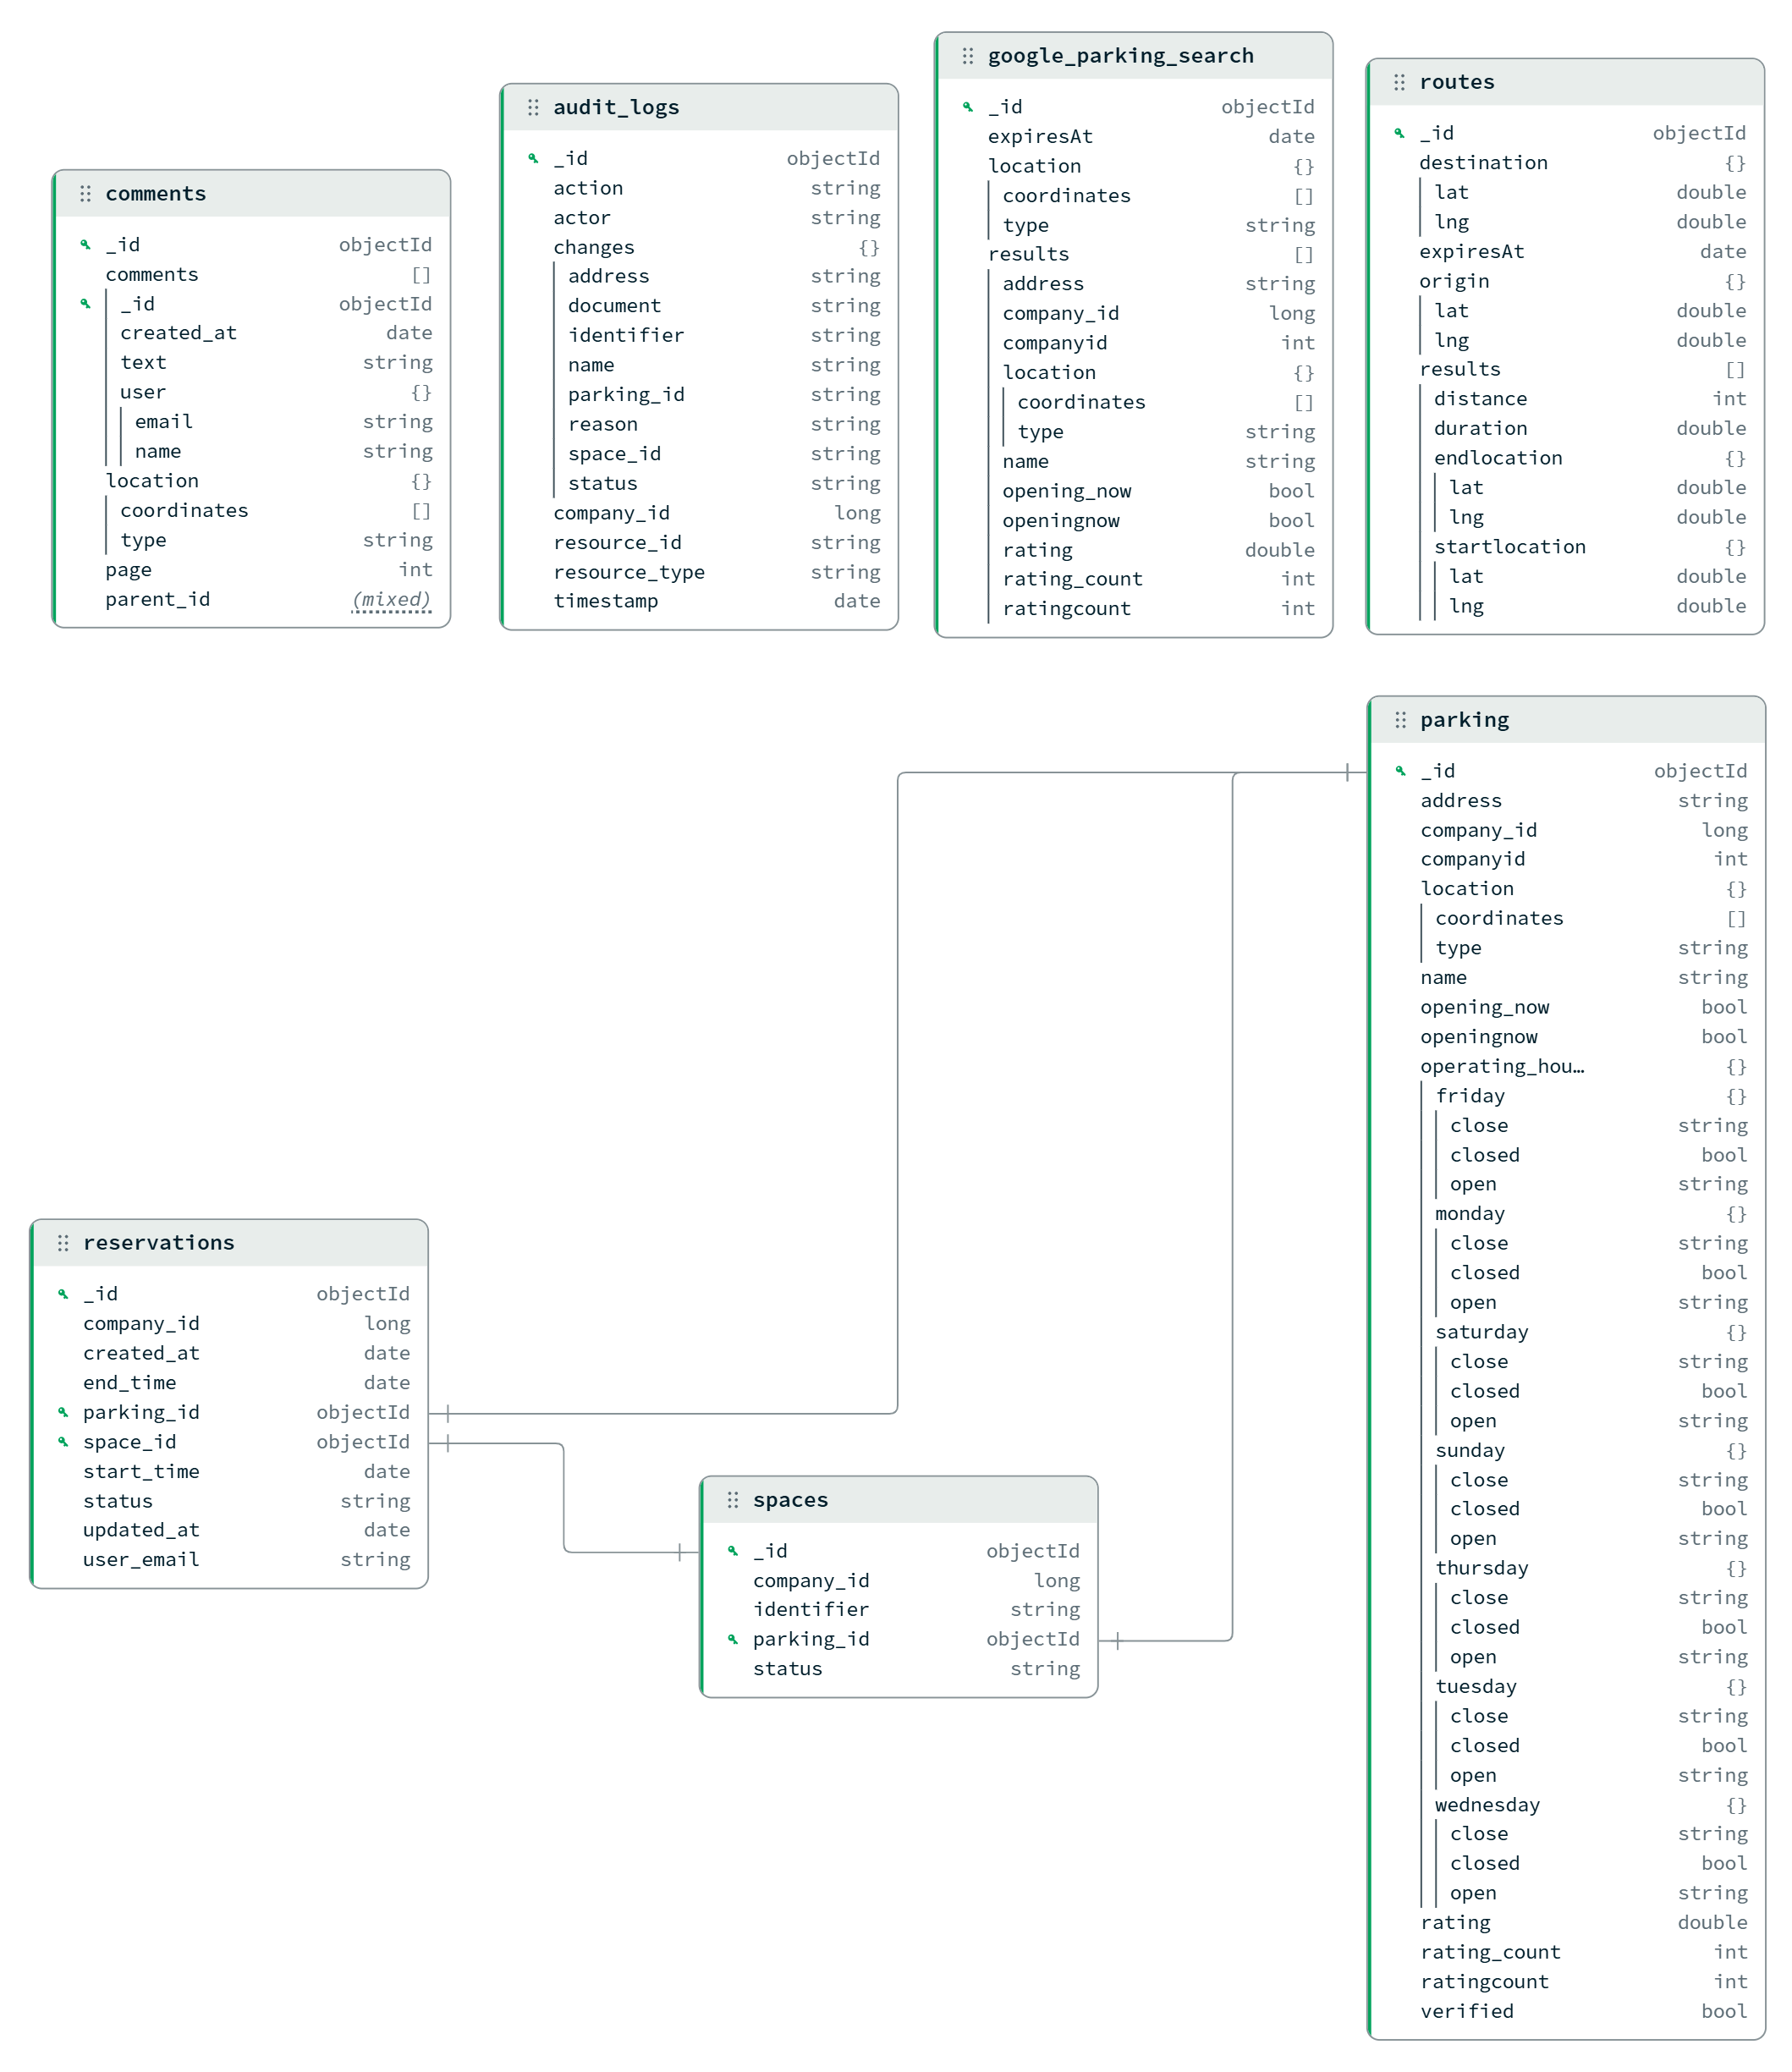
\includegraphics[width=0.95\linewidth]{capitulos/figuras/modelo-mongo.png}
   \caption{Modelo de dados MongoDB}
   \label{fig:modelo-mongo}
\end{figure}

\begin{figure}[H]
   \centering
   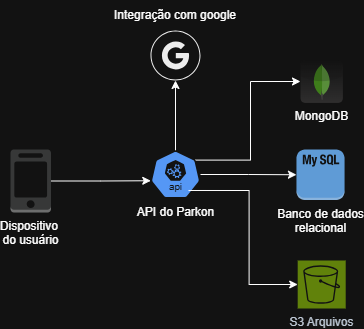
\includegraphics[width=0.55\linewidth]{capitulos/figuras/arquitetura-integracao.png}
   \caption{Arquitetura de integração da aplicação}
   \label{fig:arquitetura-integracao}
\end{figure}
